\documentclass[math, info, english]{cours}

\title{Deriving Geodesics on a 3D Mesh from the Heat Equation}
\author{Matthieu Boyer}
\def\mF{\mathcal{F}}
\def\mV{\mathcal{V}}

\begin{document}
\bettertitle

\emph{Acknowledgement: I have reused a lot of the structure of \cite{heatgeodesics} as I find their article well thought and clear.}

\begin{figure}[h]
	\centering
	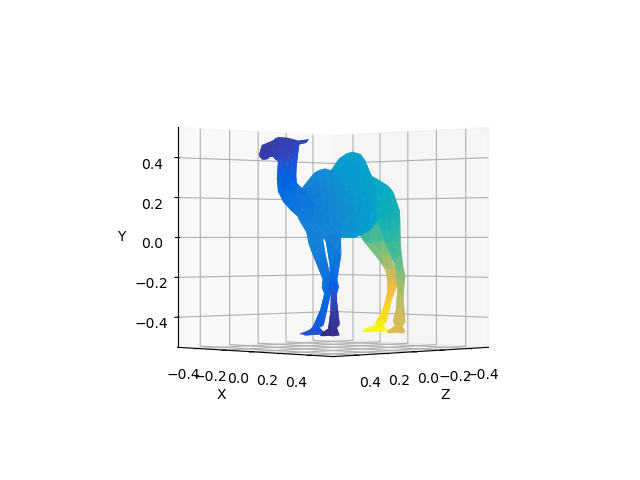
\includegraphics[width=\textwidth]{Figures/camel_t=10_i=100_False.png}
	\caption{An application of our method: a dromedary stepping on a hot rock}
\end{figure}

\section{Introduction}
Let us all remember our beloved heat equation:
\begin{equation}
	\Delta H = \frac{\partial}{\partial t} H
\end{equation}
This simple partial derivative equation encompasses the spreading of heat over time and can be described using the \emph{heat kernel}, $k_{t, x}(y)$ which measures the heat transferred from a source $x$ to a target $y$ after time $t$.
We can explicitely derive the heat kernel on $\R^{n}$ to be:
\begin{equation}
	k_{t, x}(y) = \left( 4\pi t \right)^{-n/2}\exp\left( -\frac{1}{4t} \norm{x - y}^{2}\right)
\end{equation}
which leads to a particular setting of the Varadhan's formula, linking geodesics to the heat kernel.
Indeed, in the euclidean space $\R^{n}$, the geodesic metric $d_{\R^{n}}\left( x, y \right)$ is defined by $\norm{x - y}$ for the euclidean norm.
The geodesic metric between $x$ and $y$ is the length of the shortest path (the geodesic) between $x$ and $y$ on our manifold.
In 1967, Varadhan showed the following:
\begin{thm}[\cite{varadhan}]
	If $(M, g)$ is a complete Riemannian manifold, and $k_{t, x}(y)$ is the associated heat kernel, converging to $\delta_{x}(y)$ at small times, then:
	\begin{equation}
		\tag{VF}
		-4t \log k_{t, x}(y) \xrightarrow[t \to 0]{} d\left( x, y \right)^{2}
		\label{varadhanformula}
	\end{equation}
	where $d$ is the distance function on the manifolds.
	\label{thm:varadhan}
\end{thm}
This equation comes, intuitively, from the fact that a solution of the heat equation spreads in a characteristic time $t$ along a characteristic distance $d$ will, numerically, verify $t \propto d^{2}$.
The main idea we will present here, developed in \cite{heatgeodesics} is that looking at a manifold is, numerically, the same as looking at a triangulation of the manifold, and that we can thus approximate the geodesics on our object by solving the heat equation.

\section{Related Work and Applications}
\subsection{Computing Distances}
Other ways to approach distance computations have already been tried.
The most widely used approach is solving the eikonal equation
\begin{equation}
	\norm{\nabla \phi} = 1 \text{ subject to boundary conditions } \phi_{\mid \gamma} = 0
\end{equation}
but this leads to a nonlinear and hyperbolic formulation, rendering it difficult to solve directly.
Algorithms solving the equation on implicit surfaces such as the Gauss-Seidel scheme for solving linear systems,
using fast marching and fast weeping work in $\O(n\log n)$ and $\O(n)$ but do not reuse information,
as the distance from different subsets $\gamma$ is computed from scratch each time,
leading to greater amortized costs than what we will be able to achieve here.

It is important to note that a method developed in \cite{schrod} using a time-independent version of the Schrödinger's equation
resembles a lot our method, though their computation is limited to regular grids and $R^{n}$ where solutions take a
special form, and it needs an abitrary precision on Planck's constant to determine accurate.

\subsection{Applications}
Determining the geodesic metric has applications in multiple domains.
For example, in \cite{geodesicmetricuse}, Lantuejoul and Beucher present multiple applications of the geodesic metric to image analysis.
They suggest a method to reconstruct particles and create skeletons using the geodesic distance which provides an easier time dealing with connectivity problems.
In \cite{Peyré2009}, applications of the geodesic metric are proposed to the $A^{*}$ algorithm and heuristically driven propagation as well as meshing applications.
In more industrial applications, the computer-aided-design software Solidworks possesses a geodesic offset tool, to help designer add curves and decals to their models.

\section{The Method}
Let us first describe our method in terms of smooth manifolds, we will explore computation aspects in the next sections.
This gives us algorithm \ref{heatmethod}.
\begin{algorithm}
	\caption{The Heat Method}
	\label{heatmethod}
	\begin{enumerate}
		\item Integrate $\dot{u} = \Delta u$ for some fixed time $t$.
		\item Evaluate the vector field $X = \frac{-\nabla u}{\norm{\nabla u}}$.
		\item Solve the Poisson equation $\Delta \phi = \nabla \cdot X$.
	\end{enumerate}
\end{algorithm}

$\phi$ approximates geodesic distance, approaching the true distance as $t$ goes to zero.
Since solutions to the Poisson equation are unique up to a constant, we simply make it so the smallest distance is $0$.
The initial conditions $u_{0}$ allow us to compute the distance to a single source point $x \in M$ by setting $u_{0} = \delta(x)$ and to any piecewise submanifold $\gamma$ by taking its generalized Dirac.


To prove the correction of the algorithm, remember the eikonal equation tells us that the gradient of the true geodesic metric is of unit norm.
Then, if we know the gradient of our heat approximation $\nabla u_{t}$ points in the right direction (parallel to $\nabla\phi$), we just need to solve $\Delta \phi = \nabla \cdot \frac{-\nabla u}{\norm{\nabla u}}$ to compute the distances.

However, our algorithm will not provide accurate results for now, if we do not add ways to discretize both time and space.

\subsection{Discretizing Time}
In practice, we cannot directly integrate the heat equation for step 1 of the heat method.
Thus, to simplify the calculations for ourselves, we discretize the equation using a backward Euler step for a certain time step $t$.
Thus, integrating the heat equation amounts to solving:
\begin{equation}
	\left( \id - t\Delta \right)u_{t} = u_{0}
\end{equation}
over the entire domain $M$, where $\id$ is the identity function (spatial discretization will be discussed in the next subsection).

Then, looking back at the problem of computing distances from $x$, that is $u_{0} = \delta(x)$ or:
\begin{equation}
	\tag{BP}
	\begin{array}{rcl}
		\left( \id - t\Delta \right)v_{t} = 0 & \rm on & M\setminus \{x\}\\
		v_{t} = 1 & \rm on & x
	\end{array}
	\label{boundaryproblem}
\end{equation}
as established by Varadhan in is proof of \ref{varadhanformula}, we get
\begin{equation}
	\tag{$\delta t$}
	-\frac{\sqrt{t}}{2}\log v_{t} \underset{t \to 0}{=} \phi
	\label{discretetime}
\end{equation}
which proves the correction of the algorithm with the implicit backward Euler step.

\subsection{Discretizing Space}
The method can be applied to any domain with a discrete gradient $\nabla$, divergence $\nabla \cdot$ and Laplacian $\Delta$.
As I've only considered simplicial meshes embedded in $\R^{3}$ in the implementation, since I wanted to focus on the graphics part, this is the only discretization we will look at in this theory part.
Let $M$ here be a simplicial complex represented by a triangulation $\left(\mV, \mF \subseteq \mV^{3}\right)$.
We will first remember the expressions of a few operators.
For this purpose, let $u \in \R^{\abs{V}}$ be a piecewise linear function.
The gradient of $u$ in a given triangle $f$ is:
\begin{equation}
	\nabla_{f} u = \frac{1}{2A_{f}}\sum_{i \in f} u_{i}\left( N \land e_{j_{i}} \right)
\end{equation}
where $A_{f}$ is the area of the face, $N$ is its unit normal, $e_{j_{i}}$ is the edge vector of the face opposite to vertex $i$, oriented counter clockwise, and $u_{i}$ is the value of $u$ at vertex $i$.
To store the gradient, we can also see it as a $3\abs{\mF} \times \abs{\mV}$ sparse matrix (since it's actually $3$, $\abs{\mF}\times \abs{\mV}$ matrices).
If we denote $\vec{Je_{j_{i}}}$ the vector $N \land e_{j_{i}}$ (which is the vector $e_{j_{i}}$ rotated to point inside the face):
\begin{equation}
	\begin{aligned}
		\left(\tilde{\nabla}\right)_{i, j} =& \left( \vec{Je_{j_{i}}} \right)_{1}\\
		\left(\tilde{\nabla}\right)_{i + \abs{\mF}, j} =& \left( \vec{Je_{j_{i}}} \right)_{2}\\
		\left(\tilde{\nabla}\right)_{i + 2\abs{\mF}, j} =& \left( \vec{Je_{j_{i}}} \right)_{3}
	\end{aligned}
\end{equation}
Here we actually didn't compute the gradient but only the sum part of the operator, we then have
\begin{equation}
	\nabla = \frac{1}{2A}\tilde{\nabla}
\end{equation}
where:
\begin{equation}
	\frac{1}{2A}_{f + k\abs{\mF}, f + k\abs{\mF}} = 1 / 2\norm{e_{f_{1}} \times e_{f_{2}}}
\end{equation}
is a diagonal square matrix of size $3\abs{\mF}$ whose coefficients are defined as above for $0 \leq k \leq 2$.

Then, we can compute the divergence operator's matrix as the transpose of the gradient for the face area dot product:
\begin{equation}
	\nabla\cdot = \nabla^{T}A
\end{equation}
where $A$ is defined as previously as a $3\abs{\mF}$ diagonal matrix containing the areas of the faces.
Then, we can easily compute the laplacian operator as the composition of the gradient and the divergence:
\begin{equation}
	\Delta = \nabla \cdot \nabla = \nabla^{T}A\nabla
\end{equation}
which is coherent with the expression we might derive directly:
\begin{equation}
	\left( Lu \right)_{i} = \frac{1}{2VA_{i}}\sum_{j \in \mathcal{N}\left( i \right)}\left( \cot\alpha_{i, j} + \cot\beta_{i, j} \right)\left( u_{j} - u_{i} \right)
\end{equation}
where $VA_{i}$ is a third of the sum of all triangles incident on vertex $i$, the sum is taken over neighboring vertices and $\alpha_{i, j}, \beta_{i, j}$ are the angles opposing the corresponding edge.
We will call $L_{C}$ the sum part of this operator.
Then, retrieving our distance function amounts to solving: $\left(VA - tL_{C}\right)u = u_{0}$ and then $L_{C}\phi = \nabla\cdot \left( \frac{-\nabla u}{\norm{\nabla u}} \right)$.

\subsection{Time Step}\label{sectime}
The accuracy of our method relies on the choice of time step $t$.
Equation \ref{discretetime} tells us that having $t \to 0$ will lead us to better accuracy, when space is supposed continuous.
However, when we discretize space, we see that the limit solution to the boundary problem \ref{boundaryproblem} will be a function of the combinatorial distance, independent on our Laplacian discretization:
\begin{thm}
	Let $G = \left( V, E \right)$ be the graph induced by the sparsity pattern of any real symmetric matrix $A$, and consider the linear system:
	\begin{equation*}
		\left( \Id - t A \right)u_{t} = \delta
	\end{equation*}
	where $\delta$ is a Kronecker delta at a source vertex $u \in V$ and $t > 0$.
	Then, generically:
	\begin{equation*}
		\boxed{\phi = \lim_{t \to 0} \frac{\log u_{t}}{\log t}}
	\end{equation*}
	where $\phi \in \N^{\abs{V}}$ is the graph distance between each vertex $v \in V$ and the source vertex $u$.
	\label{thmcombi}
\end{thm}
\begin{proof}
	Let $\sigma$ be the operator norm of $A$.
	Then, for $t < \frac{1}{\sigma}$, $B = I - tA$ is invertible and we have:
	\begin{equation*}
		u_{t} = \sum_{k = 0}^{\infty} t^{k}A^{k}\delta
	\end{equation*}
	Let $v \in V$ be $n$ edges away from $u$ and consider $r_{t} = \abs{R_{v}}/\abs{s_{v}}$ where:
	\begin{equation*}
		s_{v} = \left( t^{n}A^{n}\delta \right)_{v} \neq 0, \qquad R_{v} = \left( \sum_{k = n + 1}^{\infty}t^{k}A^{k}\delta \right)_{v}
	\end{equation*}
	Since:
	\begin{equation*}
		\abs{s} \leq \sum_{k \geq n + 1} t^{k}\norm{A^{k}\delta} \leq \sum_{k \geq n + 1}t^{k}\sigma^{k}
	\end{equation*}
	and thus:
	\begin{equation*}
		r_{t} \leq \frac{t^{n + 1}\sigma^{n + 1}\sum_{k = 0}^{+\infty}t^{k}\sigma^{k}}{t^{n}\left( a^{n}\delta \right)_{v}} = c\frac{t}{1 - t\sigma}
	\end{equation*}
	where $c = \sigma^{n + 1}/\left( A^{n}\delta \right)_{v}$ does not depend on $t$.
	Therefore, $\lim_{t \to 0}r_{t}$, that is, only the first term $s_{0}$ is significant as $t$ goes to zero.
	Moreover:
	\begin{equation*}
		\log s_{0} = n\log t + \log \left( A^{n}\delta \right)_{v}
	\end{equation*}
	is dominated by the first term as $t$ goes to $0$ hence $\log \left( u_{t} \right)_{v} / \log t$ approaches $n$, the combinatorial distance on the graph.
\end{proof}

Therefore only edge proximity is influential on the accuracy of our mesh, when $t \to 0$.
We will provide an estimation on how so much this is true in the next section.
To find an optimal expression $t^{*}$ is difficult, and we thus use an estimate $t = h^{2}$ where $h$ is the expectation of the length of an edge.

\section{Implementation and Results}
In this section, we will look at the implementation and efficiency of the heat method on manifolds embedded in the 3D-space.

\subsection{Difficulties in Complexity}
Implementation for this project was done in python. We used \texttt{OFF} to represent our objects.
The implementation follows the steps detailed in the proof of correction for the algorithm on triangulated meshes.
When importing the object, we create its set of faces and vertices, and use the formulas derived earlier to compute its gradient, divergence and laplacian operators.
We will denote by $m$ the number of faces and $n$ the number of vertices.
Each operation needed to compute the gradient is done in $\O(m)$, as there are always three vertices per face, and we assume our mesh to be connected.
Then, while the complexity of our matrix product has not been increased, the use of a sparse matrix representation allows for the operations of our $3\abs{\mF} \times \abs{\mV}$ matrices to be multiplied in $\O\left( \abs{mF}^{\omega} \right)$ as $\abs{\mF} = \Theta\left( \abs{\mV} \right)$ and especially allows our space complexity to stay in $\O\left( \abs{\mF}\abs{\mV} \right)$.
Indeed, some of our meshes have up to $50\times 10^{3}$ vertices, leading to $150000 \times 150000$ matrices of floats using a good precision to occupy over $22.5$ GB if not sparsified, which goes to $7.5$ GB when considering three full matrices and about $2.5$ GB when sparsified.

While the asymptotic complexity of our algorithm is simply in $\O\left( \abs{\mF}^{2} \right)$ using $\O\left( \abs{\mF}\abs{\mV} \right)$ space, the difficulties encountered are taken into account when factoring the precision
needed on the mesh for accuracy: the distance obtained by the heat method is approximately the combinatorial weighted distance for smaller values of $t$.
Thus, having a fine mesh is a necessity for our method to be precise, which leads to larger and larger computation times.

Moreover, testing the implementation proved far more difficult than predicted, as computing by hand gradients and laplacians on graphs is quite a stretch.

\subsection{Results}
\subsubsection{Computation Time}
In figure \ref{computationtime} we present a plot of the time needed for the computation of the distances from the origin on the mesh defined by $\epsilon$:
\begin{align*}
	\mV = \left\{ \left( k\epsilon, k'\epsilon \right) \ \middle| \ 0 \leq k, k' \leq \frac{1}{\varepsilon} \right\}\\
	\mF = \left\{ \left( i, i + 1, i + n \right), \left( i, i + n, i + n -1 \right) \ \middle| \ i \leq \frac{1}{\epsilon^{2}} \right\} \cap \mV^{3}
\end{align*}
Here, the average distance between two connected points is thus given by:
\begin{equation*}
	h = \frac{4}{6}\epsilon + \frac{2}{6}\sqrt{2}\epsilon = \frac{2 + \sqrt{2}}{3}\epsilon \simeq 1.14 \times \epsilon
\end{equation*}
and thus $t = 1.3\epsilon^{2}$.

\begin{figure}[h]
	\centering
	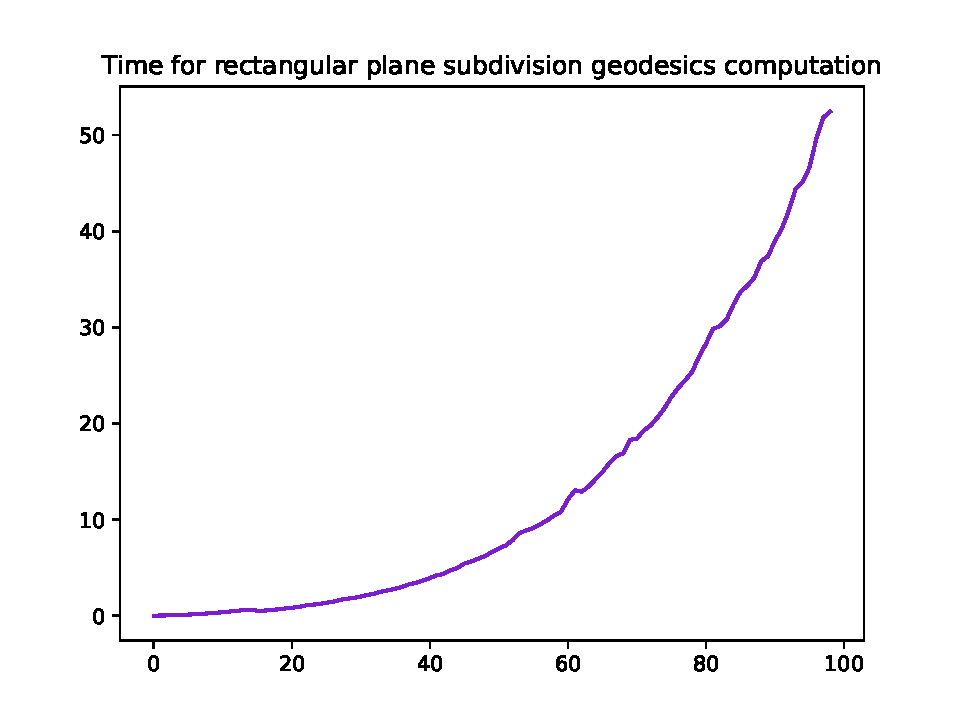
\includegraphics{Figures/tim_comp_planes_i<=100}
	\caption{Computation times for evenly spaced triangular mesh of step $1/i$ on the unit square.}
	\label{computationtime}
\end{figure}

In the above figure we can see that on iteration $i$, the number of faces is in $\O(i)$ and the complexity seems to fit in $i^{2}$.
Indeed, when computing a least squares polynomial fit, our first good fit is attained for a degree of $2$ and subsequent fits do not improve the error much as can be seen on figure \ref{polyfiterrors}.
\begin{figure}[h]
	\centering
	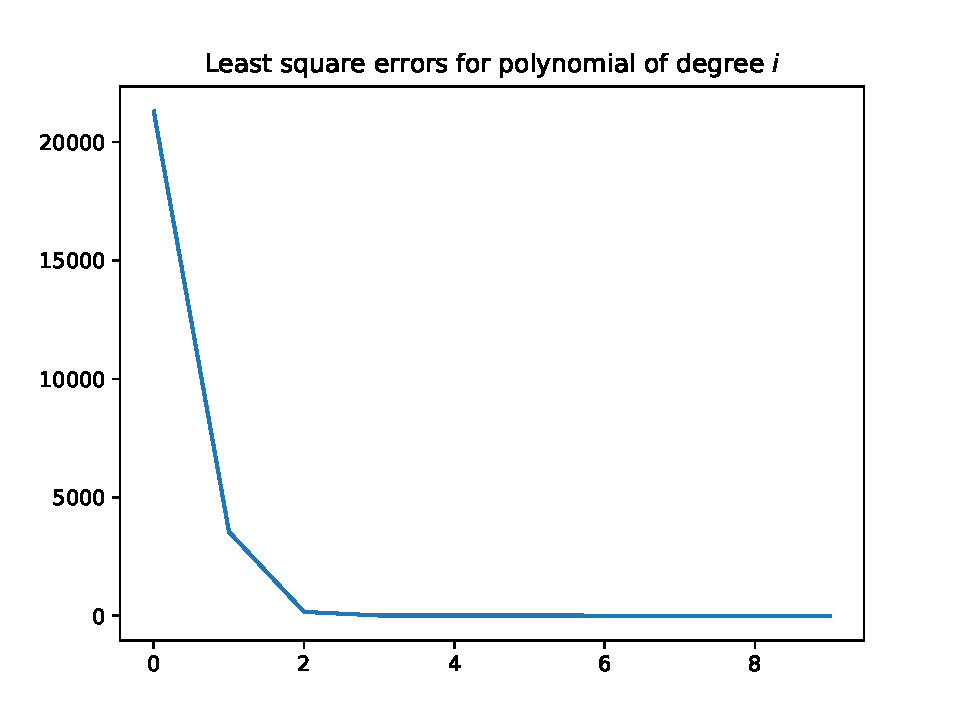
\includegraphics{Figures/polyfiterrors}
	\caption{Errors of fit for polynomials of degree up to $10$}
	\label{polyfiterrors}
\end{figure}

\subsubsection{Accuracy}
Let us take our plane mesh defined by $\epsilon$. The geodesic distance to $0$ can be directly computed:
\begin{equation*}
d\left( x \right) = \norm{x} \text{ and on indices } d_{\epsilon}\left( i \right) = \epsilon\sqrt{\left( i \mod \frac{1}{\epsilon} \right)^{2} + \left( i // \frac{1}{\epsilon} \right)^{2}}
\end{equation*}
where $//$ and $\mod$ denote the dividend and the rest respectively in the euclidean division.
\begin{figure}[H]
	\centering
	\resizebox{.5\textwidth}{.5\textwidth}{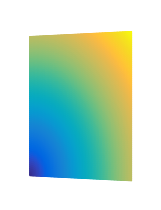
\includegraphics{Figures/plane_geodesics}}
	\caption{Illustration of the geodesic distance from $0$ on the evenly spaced mesh of step $1/70$ on the plane}
\end{figure}

We then compute the mean of difference between the theoretical distance $d$ which we just derived and the heat-method-computed geodesic metric $\tilde{d}$.

Section \ref{sectime} and Theorem \ref{thmcombi} tell us that our difference should be around the difference between $d$ and the combinatorial distance $\phi$ multplied by the step size $\epsilon$:
\begin{equation*}
	\begin{aligned}
	d\left( i \right) - \epsilon\phi\left( i \right) =& \epsilon \times
			\sqrt{\left( i \mod \frac{1}{\epsilon} \right)^{2} + \left( i // \frac{1}{\epsilon} \right)^{2} }
			-
			\epsilon \times\left( i \mod \frac{1}{\epsilon} \right) + \left(i // \frac{1}{\epsilon} \right)\\
	\leq& \frac{\epsilon}{2} \left(\left( i \mod \frac{1}{\epsilon} \right) + \left(i // \frac{1}{\epsilon} \right) \right)
	\end{aligned}
\end{equation*}

In figure \ref{planediff} we have represented the theoretical expected accuracy and actual accuracy of our method.
\begin{figure}[H]
	\centering
	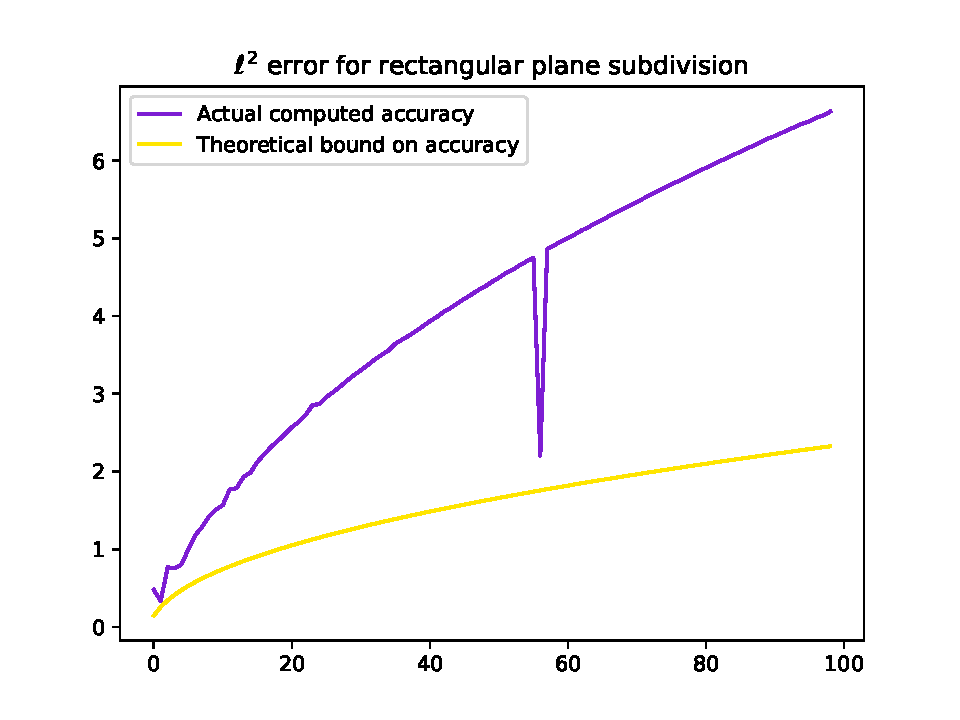
\includegraphics{Figures/compare_err_comp_planes_i<=100}
	\caption{Theoretical bound on accuracy of the heat methods for regular meshes for the plane of step $1/i$}
	\label{planediff}
\end{figure}
We can then see than, up to a constant, the plotted accuracy is the same as our theoretical bound.
The increase in the accuracy that happens at $i = 56$ could not be explained.
Why the accuracy increase in the mesh does not decrease has also not been explained.

\appendix
\newpage
\bibliography{report}
\bibliographystyle{alpha}
\end{document}
